\textbf{(DRAFT)}
Quantum error correction -- I recommend Chapter 7 of the notes from A. Ekert\footnote{The one who came up with the \texttt{Ekert91} protocol indeed!} et al: \url{https://qubit.guide/7-stabilisers}

You may also find the notes from the MMathPhys course useful: \url{https://zhenyucai.com/post/intro_to_qi/AdditionalMaterials/QECNotes.pdf}
\begin{parts}
	\part Bookwork -- to encode $\ket{\psi}$ into $\ket{\psi_L}$, we pass it through the network below:
	\begin{figure}[H]
		\centering
		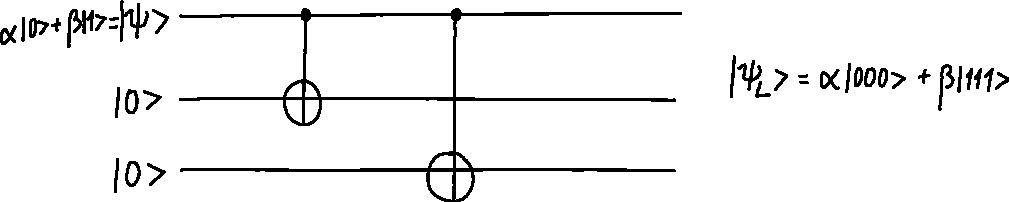
\includegraphics[width=.75\linewidth]{q4-encode}
	\end{figure}
	
	To decode, we simply reverse the network:
	\begin{figure}[H]
		\centering
		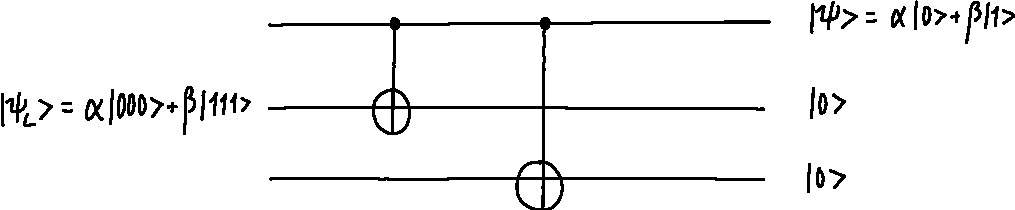
\includegraphics[width=.75\linewidth]{q4-decode}
	\end{figure}
	
	\part For a logical qubit $\ket{\psi_L} = \alpha\ket{0_L} + \beta\ket{1_L} = \alpha\ket{000} + \beta\ket{111}$, the following bit-flips are possible:
	
	\begin{itemize}
		\item 0 bit flips
		
		In this case we simply have $\ket{\psi_L} = \alpha\ket{000} + \beta\ket{111}$ with a probability of $(1-p)^3$.
		
		\item 1 bit flip
		
		Three cases arise.
		\begin{equation*}
			\ket{\psi_L} =
			\begin{cases}
				\alpha\ket{001} + \beta\ket{110} \textnormal{\hspace{1em}3rd qubit flips} \\
				\alpha\ket{010} + \beta\ket{101} \textnormal{\hspace{1em}2nd qubit flips} \\
				\alpha\ket{100} + \beta\ket{011} \textnormal{\hspace{1em}1st qubit flips}
			\end{cases}
		\end{equation*}
		Each of which has a probability of $p(1-p)^2$ occurring.
		
		\item 2 bit flips:
		Similar to the 1 bit flip case.
		\begin{equation*}
			\ket{\psi_L} =
			\begin{cases}
				\alpha\ket{011} + \beta\ket{100} \textnormal{\hspace{1em}2nd and 3rd qubits flip} \\
				\alpha\ket{101} + \beta\ket{010} \textnormal{\hspace{1em}1st and 3rd qubits flip} \\
				\alpha\ket{110} + \beta\ket{001} \textnormal{\hspace{1em}1st and 2nd qubits flip}
			\end{cases}
		\end{equation*}
		Each of which has a probability of $p^2 (1-p)$ occurring.
		
		\item 3 bit flips:
		Similar to the 0 bit flip case, we have $\ket{\psi_L} = \alpha\ket{111} + \beta\ket{000}$ with a probability of $p^3$.
	\end{itemize}
	
	\part From the point of view of the ancillas, we are effectively measuring the parity between each physical qubit.
	\begin{figure}[H]
		\centering
		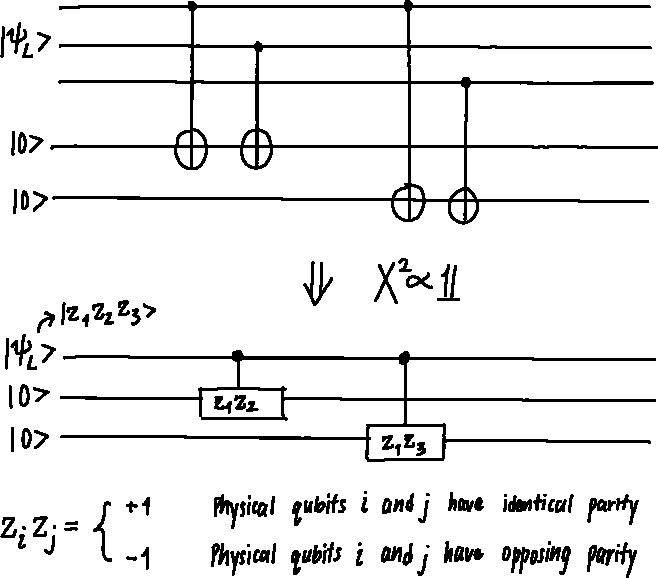
\includegraphics[width=.7\linewidth]{q4-bit-flip-code}
	\end{figure}
	
	As suggested by the diagram above, by measuring the ancillas, we may obtain the value of $z_1 z_2$ and $z_1 z_3$, which may be related to the single qubit error as follows:
	
	\begin{center}
		\begin{tabular}{|c|c|c|c|}
			\hline
			$z_1 z_2$ & $z_1 z_3$ & Physical Qubits & Correction Required \\
			\hline
			$+1$ & $+1$ & $\alpha\ket{000} + \beta\ket{111}$ & $\mathds{1}$ \\
			$+1$ & $-1$ & $\alpha\ket{001} + \beta\ket{110}$ & $\mathrm{X}_3$ \\
			$-1$ & $+1$ & $\alpha\ket{010} + \beta\ket{101}$ & $\mathrm{X}_2$ \\
			$-1$ & $-1$ & $\alpha\ket{100} + \beta\ket{011}$ & $\mathrm{X}_1$ \\
			\hline
		\end{tabular}
	\end{center}
	
	The encoded qubit is unaffected by the measurement as the operations above are of Pauli group $\mathcal{P}$ which have the properties of $\mathcal{P}^2 = \pm\mathds{1}$.
	
	One thing of note is that the table above applies to the vector space\footnote{A detour: the vector space described by a stabiliser is known as the code space. The operations we are doing here are simply to check if the qubit resides in the code space since the Pauli group guarantees the eigenvalue to be $\pm 1$.} spanned by the corresponding basis.
	Hence if there were 2 or 3 errors, we would have applied the wrong correction operation to the qubits.
	
	In the 2 bit flips case, we would have the table above with the coefficients $\alpha$ and $\beta$ swapped.
	After the erroneous correction, we will end up with the 3 bit flips case where $\ket{\psi_L} = \beta\ket{000} + \alpha\ket{111}$.
	
	This is not a significant concern as the probability of individual bit flip $p$ is usually very small, therefore a simultaneous $n$ bit flips would have a probability proportional to $p^n$ which approaches 0 quickly.
	
	\part If a Z error were to occur, the network will be unable to detect it as it only measures the parity of the $z$ component between each qubit.
	
	Conversely, if a Y error were to occur, the network will be able to detect it as we know $\mathrm{Y} = i\mathrm{Z}\mathrm{X}$, and $\pm\mathrm{Z}$ stabilises the Z basis states of $\ket{0}$ and $\ket{1}$.
	Hence an error in $\mathrm{Y}$ would contain a distinguishable error in $Z$, which can then be reliably detected by the network above.
	
	\part We also know that $\mathrm{H}\mathrm{X}\mathrm{H} = \mathrm{Z}$ where $\mathrm{H}$ is the Hadamard gate.
	Therefore to detect an Z error we simply add a pair of Hadamard gates in front and back of the \texttt{CNOT} gates.
	
	\part \textbf{(TO BE VERIFIED)}
	The table above suggests that we may construct a feedback circuit of \texttt{CNOT} gates to automatically correct the $\mathrm{X}$ error as follows:
	\begin{figure}[H]
		\centering
		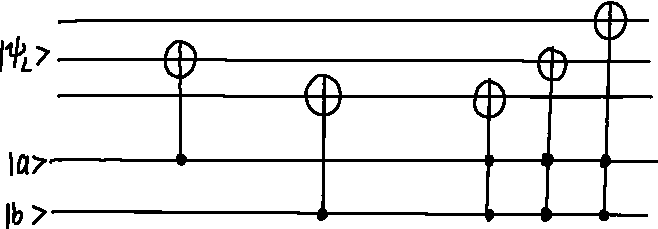
\includegraphics[width=.7\linewidth]{q4-error-correction}
	\end{figure}
	
	This approach has the advantage of not having to perform measurement on the ancillas, thereby providing greater isolation to the QEC circuit which helps in guarding against decoherence.
	However, the lack of measurement also makes the assessment of fidelity difficult as we no longer have the explicit states of the ancillas.
	
	\part Nothing to do with error correction here!
	The best description we can have for a qubit whose state is unknown due to a random process is naturally a \underline{density matrix}.
	
	So in the first case we may construct the density matrix as follows:
	\begin{align*}
		\rho_{\pm\phi} &= \frac{1}{2} \ket{\psi^{+\phi}}\bra{\psi^{+\phi}} + \frac{1}{2} \ket{\psi^{-\phi}}\bra{\psi^{-\phi}} \\
		&= \frac{1}{2} \left[
		\begin{pmatrix}
			\alpha \\ \beta \mathrm{e}^{+i\phi}
		\end{pmatrix}
		\begin{pmatrix}
			\alpha^* & \beta^* \mathrm{e}^{-i\phi}
		\end{pmatrix}
		+ \begin{pmatrix}
			\alpha \\ \beta \mathrm{e}^{-i\phi}
		\end{pmatrix}
		\begin{pmatrix}
			\alpha^* & \beta^* \mathrm{e}^{+i\phi}
		\end{pmatrix}
		\right] \\
		&= \frac{1}{2} \left[
		\begin{pmatrix}
			|\alpha|^2 & \alpha \beta^* \mathrm{e}^{-i\phi} \\
			\alpha^* \beta \mathrm{e}^{+i\phi} & |\beta|^2
		\end{pmatrix}
		+ \begin{pmatrix}
			|\alpha|^2 & \alpha \beta^* \mathrm{e}^{+i\phi} \\
			\alpha^* \beta \mathrm{e}^{-i\phi} & |\beta|^2
		\end{pmatrix}
		\right] \\
		&= \begin{pmatrix}
			|\alpha|^2 & \alpha \beta^* \cos\phi \\
			\alpha^* \beta \cos\phi & |\beta|^2
		\end{pmatrix}
	\end{align*}
	
	And for the case where the qubit experiences a phase flip with probability $q$, we have:
	\begin{align*}
		\phi_\textnormal{Z} &= \left(1-q\right) \ket{\psi}\bra{\psi} + q \ket{\psi^\textnormal{Z}}\bra{\psi^\textnormal{Z}} \\
		&= \left(1-q\right) \begin{pmatrix}
			\alpha \\ \beta
		\end{pmatrix}
		\begin{pmatrix}
			\alpha^* & \beta^*
		\end{pmatrix}
		+ q \begin{pmatrix}
			\alpha \\ -\beta
		\end{pmatrix}
		\begin{pmatrix}
			\alpha^* & -\beta^*
		\end{pmatrix} \\
		&= \left(1-q\right) \begin{pmatrix}
			|\alpha|^2 & \alpha \beta^* \\
			\alpha^* \beta & |\beta|^2
		\end{pmatrix}
		+ q \begin{pmatrix}
			|\alpha|^2 & -\alpha \beta^* \\
			-\alpha^* \beta & |\beta|^2
		\end{pmatrix} \\
		&= \begin{pmatrix}
			|\alpha|^2 & \left(1-2q\right) \alpha \beta^* \\
			\left(1-2q\right) \alpha^* \beta & |\beta|^2
		\end{pmatrix}
	\end{align*}
	
	Comparing the terms simply yields:
	\begin{gather*}
		1-2q = \cos\phi \\
		\Rightarrow q = \frac{1-\cos\phi}{2}
	\end{gather*}
\end{parts}